\documentclass[10pt,twocolumn]{article}
\usepackage[margin=0.70in,columnsep=0.35in]{geometry}
\usepackage{amsmath,amssymb}
\usepackage{graphicx}
\usepackage{booktabs}
\usepackage[colorlinks=true,linkcolor=blue,citecolor=blue,urlcolor=blue]{hyperref}
\usepackage{orcidlink}
\usepackage{microtype}
\usepackage{caption}
\captionsetup{font=small,labelfont=bf}

\title{\textbf{Fluorine Multiple Bonding in Monofluoride Cations: A Relativistic All-Electron Audit}}

\author{Julian~M.~Kleber\,\orcidlink{0000-0001-5518-0932}\\
\small Independent researcher, Berlin, Germany}
\date{November 21, 2026}

\begin{document}
% Auto-generated by scripts/emit_manuscript_macros.py — do not edit by hand.
% Regenerate: python scripts/emit_manuscript_macros.py

\newcommand{\DataCFplusBO}{1.854}
\newcommand{\DataCFplusreang}{1.1596}
\newcommand{\DataDesignCFplusBOpbe}{1.985}
\newcommand{\DataDesignCFplusHFbo}{1.819}
\newcommand{\DataDesignCFplusHFpi}{0.939}
\newcommand{\DataDesignCFplusSigPi}{0.88/1.09}
\newcommand{\DataDesignCFplusqF}{+0.74}
\newcommand{\DataDesignCFplusre}{1.1532}
\newcommand{\DataDesignCrFfiveplusBOpbe}{0.767}
\newcommand{\DataDesignCrFfiveplusHFbo}{0.313}
\newcommand{\DataDesignCrFfiveplusHFpi}{0.021}
\newcommand{\DataDesignCrFfiveplusSigPi}{0.49/0.21}
\newcommand{\DataDesignCrFfiveplusqF}{+1.51}
\newcommand{\DataDesignCrFfiveplusre}{2.151}
\newcommand{\DataDesignFCFtwoplusBOpbe}{2.038}
\newcommand{\DataDesignFCFtwoplusHFbo}{1.956}
\newcommand{\DataDesignFCFtwoplusHFpi}{0.973}
\newcommand{\DataDesignFCFtwoplusSigPi}{0.98/1.05}
\newcommand{\DataDesignFCFtwoplusqF}{+0.94}
\newcommand{\DataDesignFCFtwoplusre}{1.1461}
\newcommand{\DataDesignMoFfiveplusBOpbe}{2.58}
\newcommand{\DataDesignMoFfiveplusHFbo}{2.421}
\newcommand{\DataDesignMoFfiveplusHFpi}{1.495}
\newcommand{\DataDesignMoFfiveplusSigPi}{0.85/1.69}
\newcommand{\DataDesignMoFfiveplusqF}{+1.05}
\newcommand{\DataDesignMoFfiveplusre}{1.6707}
\newcommand{\DataDesignNFtwoplusBOpbe}{2.427}
\newcommand{\DataDesignNFtwoplusHFbo}{2.286}
\newcommand{\DataDesignNFtwoplusHFpi}{1.361}
\newcommand{\DataDesignNFtwoplusSigPi}{0.92/1.50}
\newcommand{\DataDesignNFtwoplusqF}{+1.05}
\newcommand{\DataDesignNFtwoplusre}{1.0859}
\newcommand{\DataDesignNbFfourplusBOpbe}{2.216}
\newcommand{\DataDesignNbFfourplusHFbo}{2.022}
\newcommand{\DataDesignNbFfourplusHFpi}{1.205}
\newcommand{\DataDesignNbFfourplusSigPi}{0.78/1.40}
\newcommand{\DataDesignNbFfourplusqF}{+0.74}
\newcommand{\DataDesignNbFfourplusre}{1.6548}
\newcommand{\DataDesignOFthreeplusBOpbe}{2.745}
\newcommand{\DataDesignOFthreeplusHFbo}{2.682}
\newcommand{\DataDesignOFthreeplusHFpi}{1.776}
\newcommand{\DataDesignOFthreeplusSigPi}{0.89/1.85}
\newcommand{\DataDesignOFthreeplusqF}{+1.46}
\newcommand{\DataDesignOFthreeplusre}{1.0784}
\newcommand{\DataDesignTaFfourplusBOpbe}{2.154}
\newcommand{\DataDesignTaFfourplusHFbo}{1.969}
\newcommand{\DataDesignTaFfourplusHFpi}{1.184}
\newcommand{\DataDesignTaFfourplusSigPi}{0.76/1.36}
\newcommand{\DataDesignTaFfourplusqF}{+0.65}
\newcommand{\DataDesignTaFfourplusre}{1.6759}
\newcommand{\DataDesignTiFthreeplusBOpbe}{2.036}
\newcommand{\DataDesignTiFthreeplusHFbo}{1.799}
\newcommand{\DataDesignTiFthreeplusHFpi}{1.027}
\newcommand{\DataDesignTiFthreeplusSigPi}{0.74/1.28}
\newcommand{\DataDesignTiFthreeplusqF}{+0.68}
\newcommand{\DataDesignTiFthreeplusre}{1.5739}
\newcommand{\DataDesignVFfourplusBOpbe}{2.486}
\newcommand{\DataDesignVFfourplusHFbo}{1.747}
\newcommand{\DataDesignVFfourplusHFpi}{0.814}
\newcommand{\DataDesignVFfourplusSigPi}{0.84/1.63}
\newcommand{\DataDesignVFfourplusqF}{+1.01}
\newcommand{\DataDesignVFfourplusre}{1.5652}
\newcommand{\DataDesignWFfiveplusBOpbe}{2.481}
\newcommand{\DataDesignWFfiveplusHFbo}{2.342}
\newcommand{\DataDesignWFfiveplusHFpi}{1.477}
\newcommand{\DataDesignWFfiveplusSigPi}{0.82/1.63}
\newcommand{\DataDesignWFfiveplusqF}{+0.91}
\newcommand{\DataDesignWFfiveplusre}{1.6764}
\newcommand{\DataDesignZrFthreeplusBOpbe}{1.844}
\newcommand{\DataDesignZrFthreeplusHFbo}{1.623}
\newcommand{\DataDesignZrFthreeplusHFpi}{0.926}
\newcommand{\DataDesignZrFthreeplusSigPi}{0.70/1.11}
\newcommand{\DataDesignZrFthreeplusqF}{+0.51}
\newcommand{\DataDesignZrFthreeplusre}{1.7097}
\newcommand{\DataMnFonedeltaEeV}{5.52}
\newcommand{\DataMnFfivedeltaEeV}{-0.245}
\newcommand{\DataMnFsevenBO}{0.617}
\newcommand{\DataMnFsevenomegacm}{606.8}
\newcommand{\DataMnFsevenqF}{-0.34}
\newcommand{\DataMnFsevenreang}{1.8341}
\newcommand{\DataMoFfiveplusBOpbe}{2.5796}
\newcommand{\DataNFBO}{1.058}
\newcommand{\DataNFpiBO}{0.319}
\newcommand{\DataNFreang}{1.3136}
\newcommand{\DataOFthreeccpVDZDKBOpbe}{2.6437}
\newcommand{\DataOFthreeccpVTZDKBOpbe}{2.7446}
\newcommand{\DataOFthreeplusBOhf}{2.6816}
\newcommand{\DataOFthreeplusBOpbe}{2.7446}
\newcommand{\DataOFthreepluspipbe}{1.8495}
\newcommand{\DataOFthreeplusreang}{1.0784}
\newcommand{\DataPdFtwopfourMfourAEXtwoCccDKBO}{0.272}
\newcommand{\DataPdFtwopfourMfourAEXtwoCccDKomega}{323}
\newcommand{\DataPdFtwopfourMfourAEXtwoCccDKpi}{0.039}
\newcommand{\DataPdFtwopfourMfourAEXtwoCccDKqF}{+0.34}
\newcommand{\DataPdFtwopfourMfourAEXtwoCccDKre}{2.1054}
\newcommand{\DataPdFtwopfourMfourAEXtwoCccDKsigma}{0.223}
\newcommand{\DataPdFtwopfourMfourAEXtwoCxtwocTZBO}{0.233}
\newcommand{\DataPdFtwopfourMfourAEXtwoCxtwocTZomega}{286}
\newcommand{\DataPdFtwopfourMfourAEXtwoCxtwocTZpi}{0.025}
\newcommand{\DataPdFtwopfourMfourAEXtwoCxtwocTZqF}{+0.25}
\newcommand{\DataPdFtwopfourMfourAEXtwoCxtwocTZre}{2.1467}
\newcommand{\DataPdFtwopfourMfourAEXtwoCxtwocTZsigma}{0.208}
\newcommand{\DataPdFtwopfourMfourECPccPPBO}{0.274}
\newcommand{\DataPdFtwopfourMfourECPccPPomega}{310}
\newcommand{\DataPdFtwopfourMfourECPccPPpi}{0.038}
\newcommand{\DataPdFtwopfourMfourECPccPPqF}{+0.33}
\newcommand{\DataPdFtwopfourMfourECPccPPre}{2.1232}
\newcommand{\DataPdFtwopfourMfourECPccPPsigma}{0.227}
\newcommand{\DataPdFtwopfourMfourECPdeftwoBO}{0.223}
\newcommand{\DataPdFtwopfourMfourECPdeftwoomega}{286}
\newcommand{\DataPdFtwopfourMfourECPdeftwopi}{0.035}
\newcommand{\DataPdFtwopfourMfourECPdeftwoqF}{+0.24}
\newcommand{\DataPdFtwopfourMfourECPdeftwore}{2.1422}
\newcommand{\DataPdFtwopfourMfourECPdeftwosigma}{0.186}
\newcommand{\DataPdFtwoMtwoAEXtwoCccDKBO}{0.609}
\newcommand{\DataPdFtwoMtwoAEXtwoCccDKomega}{584}
\newcommand{\DataPdFtwoMtwoAEXtwoCccDKpi}{0.167}
\newcommand{\DataPdFtwoMtwoAEXtwoCccDKqF}{-0.36}
\newcommand{\DataPdFtwoMtwoAEXtwoCccDKre}{1.9005}
\newcommand{\DataPdFtwoMtwoAEXtwoCccDKsigma}{0.428}
\newcommand{\DataPdFtwoMtwoAEXtwoCxtwocTZBO}{0.45}
\newcommand{\DataPdFtwoMtwoAEXtwoCxtwocTZomega}{562}
\newcommand{\DataPdFtwoMtwoAEXtwoCxtwocTZpi}{0.096}
\newcommand{\DataPdFtwoMtwoAEXtwoCxtwocTZqF}{-0.50}
\newcommand{\DataPdFtwoMtwoAEXtwoCxtwocTZre}{1.914}
\newcommand{\DataPdFtwoMtwoAEXtwoCxtwocTZsigma}{0.351}
\newcommand{\DataPdFtwoMtwoECPccPPBO}{0.601}
\newcommand{\DataPdFtwoMtwoECPccPPomega}{589}
\newcommand{\DataPdFtwoMtwoECPccPPpi}{0.164}
\newcommand{\DataPdFtwoMtwoECPccPPqF}{-0.37}
\newcommand{\DataPdFtwoMtwoECPccPPre}{1.9116}
\newcommand{\DataPdFtwoMtwoECPccPPsigma}{0.425}
\newcommand{\DataPdFtwoMtwoECPdeftwoBO}{0.397}
\newcommand{\DataPdFtwoMtwoECPdeftwoomega}{571}
\newcommand{\DataPdFtwoMtwoECPdeftwopi}{0.085}
\newcommand{\DataPdFtwoMtwoECPdeftwoqF}{-0.54}
\newcommand{\DataPdFtwoMtwoECPdeftwore}{1.9197}
\newcommand{\DataPdFtwoMtwoECPdeftwosigma}{0.309}
\newcommand{\DataPdFtwoplusfourAEccDKmayerpi}{0.039}
\newcommand{\DataPdFtwoplusfourAEccDKmayersigma}{0.223}
\newcommand{\DataSuperacidOsOFplusCvdOsVIIIBO}{1.024}
\newcommand{\DataSuperacidOsOFplusCvdOsVIIISigPi}{0.66/0.34}
\newcommand{\DataSuperacidOsOFplusCvdOsVIIIqF}{-0.09}
\newcommand{\DataSuperacidOsOFplusCvdOsVIIIre}{1.79}
\newcommand{\DataSuperacidReFplusOhdReVIIBO}{1.2119}
\newcommand{\DataSuperacidReFplusOhdReVIISigPi}{0.57/0.59}
\newcommand{\DataSuperacidReFplusOhdReVIIqF}{-0.03}
\newcommand{\DataSuperacidReFplusOhdReVIIre}{1.7846}
\newcommand{\DataSuperacidTiFplusBFneutralpairBO}{1.0388}
\newcommand{\DataSuperacidTiFplusBFneutralpairSigPi}{0.46/0.56}
\newcommand{\DataSuperacidTiFplusBFneutralpairqF}{-0.11}
\newcommand{\DataSuperacidTiFplusBFneutralpairre}{1.7311}
\newcommand{\DataSuperacidWFplusBFneutralpairBO}{1.1872}
\newcommand{\DataSuperacidWFplusBFneutralpairSigPi}{0.62/0.53}
\newcommand{\DataSuperacidWFplusBFneutralpairqF}{-0.07}
\newcommand{\DataSuperacidWFplusBFneutralpairre}{1.7899}
\newcommand{\DataWFfiveplusBOpbe}{2.4814}
\newcommand{\DataforensicbsS}{1.978}
\newcommand{\DataforensicbsdeltaeV}{-2.939}
\newcommand{\Dataforensicbsenergyha}{-1249.1697639}
\newcommand{\Dataforensicmeanuhfoffsetmha}{-31.59}

\maketitle

\begin{abstract}
Fluorine is the most electronegative element and is canonically treated as a monovalent $\sigma$-acceptor, although partial $\pi$-donation is established in $\mathrm{NF}$ and $\mathrm{CF}^+$. Building on an earlier preprint (DOI 10.26434/chemrxiv-2022-xlsjn-v3), I perform scalar-relativistic all-electron calculations of $\mathrm{CF}^+$, $\mathrm{NF}$, neutral $\mathrm{MnF}$, and high-valent $3d$/$4d$/$5d$ monofluoride cations. Main-group and $\mathrm{MnF}$ benchmarks use X2C-CASSCF/SC-NEVPT2 with \texttt{cc-pVTZ-DK}; multiply charged triple-bond candidates use X2C-PBE0 and X2C-HF at local minima, with $\sigma/\pi$-decomposed Mayer bond orders and L\"owdin charges. At this valence active space, X2C-CAS(12,9)-NEVPT2 places $^5\Sigma^+$ \emph{below} $^7\Sigma^+$ by $|\DataMnFfivedeltaEeV|\,$eV; metal $3s3p$ core--valence correlation and spin--orbit coupling remain unresolved, so the method does not reproduce the experimental $\mathrm{MnF}$ spin ordering. Where calibrated against experiment ($^7\Sigma^+$), NEVPT2 still matches $r_e$ and $\omega_e$ ($\DataMnFsevenreang$\,\AA, $\DataMnFsevenomegacm\,\mathrm{cm}^{-1}$) as a polar single bond (BO $=\DataMnFsevenBO$, $q(\mathrm{F})=\DataMnFsevenqF$). On the sampled $1.60$--$2.80\,$\AA\ grid, the lowest $^1\Sigma^+$ point lies $+\DataMnFonedeltaEeV\,$eV above the $^7\Sigma^+$ minimum (BO $= 0.893$ at the short-distance boundary, not a converged singlet minimum). A non-relativistic PySCF replay of ChemRxiv v3 singlet data uncovers a $\DataforensicbsdeltaeV\,$eV UHF broken-symmetry instability ($\langle S^2\rangle=\DataforensicbsS$). Most bare late-$3d$ trications Coulomb-explode, except the sextet $[\mathrm{MnF}]^{3+}$ metastable well. In a matched $2\times 2$ (core $\times$ basis family) audit with spin-pure AVAS-CASCI(12--15,9)/SC-NEVPT2, all four protocols agree qualitatively: $\mathrm{PdF}$ ($^2\Sigma^+$) and quartet $[\mathrm{PdF}]^{2+}$ are bound, $[\mathrm{PdF}]^{3+}$ is repulsive; earlier apparent binding reversals were artefacts of spin-uncontrolled CASSCF. Screening identifies metastable local minima with high Mayer $\sigma+\pi$ indices, e.g.\ $\DataOFthreeplusBOpbe$ ($\pi=\DataOFthreepluspipbe$) in $[\mathrm{OF}]^{3+}$ and $\DataMoFfiveplusBOpbe$--$\DataWFfiveplusBOpbe$ in $[\mathrm{MoF}]^{5+}$/$[\mathrm{WF}]^{5+}$, without thermodynamic or lifetime claims.
\end{abstract}

\section{Introduction}
Fluorine's extreme electronegativity makes it the textbook monovalent $\sigma$-acceptor. Nevertheless, its stereochemically active lone pairs (predominantly $2p_\pi$ perpendicular to a $\sigma$ bond) can donate $\pi$-electron density toward strongly electrophilic centers \cite{frenking2000}. In main-group diatomics, partial double-bond character is established in $\mathrm{NF}$ \cite{harbison2002}, and the $14$-electron cation $\mathrm{CF}^+$ exhibits substantial $\mathrm{F}\to\mathrm{C}$ $\pi$-donation. Whether fluorine can form triple bonds with transition metals was explored qualitatively in an earlier ChemRxiv preprint \cite{kleber2025}.

Three concrete goals motivate this quantitative revision. First, I investigate the spin-state ordering and bonding of neutral $\mathrm{MnF}$, where matrix-isolation IR \cite{brosi2016}, ESR \cite{devore1978}, rotational spectroscopy \cite{sheridan2003}, and prior ab initio studies \cite{koukounas2004} establish a $X\,^7\Sigma^+$ ground state, and I audit the SCF reproducibility anomalies of the earlier preprint \cite{seeger1977}. Second, I audit spin-pure matched all-electron versus ECP protocols \cite{weigend2005,pyykko2012,peterson2007} on oxidized $4d$ palladium fluorides. Third, guided by highest-oxidation-state chemistry \cite{riedel2009}, I rationally screen $10$-valence-electron main-group and $d^0$ transition-metal cations for local minima with elevated Mayer $\sigma+\pi$ indices.

\section{Computational Methods}
All calculations were executed in open-source PySCF 2.15.1 \cite{sun2020} (Python 3.12; software versions and BLAS metadata are archived with each results bundle in the repository). Legacy multireference scans in \texttt{run\_ab\_initio.py} use ROHF with \texttt{max\_cycle}$=250$, \texttt{level\_shift}$=0.25$, DIIS space $=12$, and Newton fallback on failed convergence; CASSCF macro-iterations use \texttt{conv\_tol}$=10^{-6}$ and up to $60$ cycles. The palladium matched audit (\texttt{scripts/pd\_matched\_v3/}) uses density-followed, stability-checked X2C ROHF; AVAS on Pd $4d$, Pd $5s$, and F $2p$ (threshold $0.2$; \texttt{minao} guess \texttt{ano} for all-electron Pd, \texttt{minao} for ECP Pd); CASCI with three roots, \texttt{fix\_spin\_}(shift $0.5$, target $\langle S^2\rangle$), and SC-NEVPT2 on each root; curves follow the lowest spin-pure root envelope on a $1.55$--$3.20\,$\AA\ grid plus $5.00\,$\AA\ with forward/backward sweeps. Pd bases are \texttt{cc-pVTZ-PP}+ECP28MDF, \texttt{cc-pVTZ-DK}, x2c-TZVPall, and \texttt{def2-TZVP} (ECP28) \cite{peterson2007,weigend2005,andrae1990,pollak2017}; F uses matching all-electron bases (no fluorine ECP exists; the PySCF \texttt{def2-TZVP} warning is harmless). Other multireference surfaces used exact two-component (X2C) scalar-relativistic ROHF, CASSCF, and strongly contracted SC-NEVPT2 \cite{angeli2001} with the all-electron relativistic \texttt{cc-pVTZ-DK} basis set \cite{balabanov2005}. Active spaces included metal valence $d,s$ and fluorine $2p$ orbitals: CAS(8,8) for $\mathrm{CF}^+$, CAS(10,8) for $\mathrm{NF}$, CAS(12,9) for $\mathrm{MnF}$, CAS(9,9) for $[\mathrm{MnF}]^{3+}$, CAS(15,9) for $\mathrm{NiF}/\mathrm{PdF}$, CAS(13,9) for $[\mathrm{NiF}]^{2+}/[\mathrm{PdF}]^{2+}$, and CAS(12,9) for $[\mathrm{NiF}]^{3+}/[\mathrm{PdF}]^{3+}$. The CAS(12,9) $\mathrm{MnF}$ manifold omits Mn $3s3p$ core--valence correlation and spin--orbit coupling, which are required for correct $^7\Sigma^+$ versus $^5\Sigma^+$ ordering \cite{koukounas2004}.

Equilibrium bond lengths $r_e$ and harmonic frequencies $\omega_e$ were obtained from local polynomial fits (up to quartic, five-point windows) around each bound NEVPT2 minimum in \texttt{run\_ab\_initio.py}; the Pd audit uses the spin-pure envelope fits in \texttt{corrected\_summary.csv}. Covalent bond order was quantified from the CASSCF one-particle density matrix via the Mayer bond order \cite{mayer1983}, decomposed along the internuclear $z$-axis into $\sigma$ ($m_l = 0$) and $\pi$ ($|m_l| = 1$) components, alongside L\"owdin charges $q(\mathrm{F})$. Extreme triple-bond candidates were screened at X2C-PBE0 \cite{adamo1999} and cross-checked with X2C-HF using \texttt{cc-pVTZ-DK}.

\section{Results and Discussion}

\subsection{Main-Group Calibration and Neutral $\mathrm{MnF}$}
Table~\ref{tab:main_mnf} and Figure~\ref{fig:mnf} summarize the main-group calibration and the neutral $\mathrm{MnF}$ spin manifold. For $\mathrm{CF}^+$ ($^1\Sigma^+$), X2C-CAS(8,8)-NEVPT2 yields $r_e = 1.1596\,$\AA\ (expt.\ $1.154\,$\AA) and $\omega_e = 1776.8\,\mathrm{cm}^{-1}$ (expt.\ $1792\,\mathrm{cm}^{-1}$), with Mayer BO $= 1.854$ ($\pi = 1.008$, $\sigma = 0.838$, $q(\mathrm{F}) = +0.745$). Neutral $\mathrm{NF}$ ($^3\Sigma^-$) reproduces $r_e = 1.3136\,$\AA\ (expt.\ $1.317\,$\AA) with $\pi$-BO $= 0.319$ and total BO $= 1.058$.

For neutral $\mathrm{MnF}$, the $^7\Sigma^+$ surface reproduces experiment within $0.004\,$\AA\ and $1.7\,\mathrm{cm}^{-1}$ when compared at $^7\Sigma^+$ ($r_e = \DataMnFsevenreang\,$\AA\ vs.\ $1.838\,$\AA\ \cite{sheridan2003}; $\omega_e = \DataMnFsevenomegacm\,\mathrm{cm}^{-1}$ vs.\ $608.5\,\mathrm{cm}^{-1}$ in Ne \cite{brosi2016}), with Mayer BO $\DataMnFsevenBO$ and $q(\mathrm{F})=\DataMnFsevenqF$. At the same valence-only CAS(12,9)-NEVPT2 level, however, $^5\Sigma^+$ lies $\DataMnFfivedeltaEeV\,$eV \emph{below} $^7\Sigma^+$ on the grid minima (Table~\ref{tab:main_mnf}), so the \textbf{method does not reproduce the experimental spin ordering}; including semi-core correlation and spin--orbit coupling remains future work \cite{koukounas2004}. On the $1.60$--$2.80\,$\AA\ scan, the lowest sampled $^1\Sigma^+$ energy lies $+\DataMnFonedeltaEeV\,$eV above the $^7\Sigma^+$ minimum (BO $= 0.893$ at $R=1.60\,$\AA). Because the singlet minimum is not located and the method already misorders $^7\Sigma^+$ versus $^5\Sigma^+$, this scan alone does not establish the experimental ground state or exclude triple bonding.

\begin{table}[t]
\centering
\caption{X2C-CASSCF/SC-NEVPT2 (\texttt{cc-pVTZ-DK}) spectroscopic constants, Mayer bond orders ($\sigma/\pi$), and L\"owdin charges $q(\mathrm{F})$.}
\label{tab:main_mnf}
\scriptsize
\setlength{\tabcolsep}{2.0pt}
\begin{tabular}{@{}lccccccc@{}}
\toprule
Species (State) & $\langle S^2\rangle$ & $r_e$ (\AA) & $\omega_e$ ($\mathrm{cm}^{-1}$) & $\Delta E$ (eV) & BO & $\sigma/\pi$ & $q(\mathrm{F})$ \\
\midrule
$\mathrm{CF}^+$ ($^1\Sigma^+$) & $0$ & 1.1596 & 1776.8 & -- & 1.854 & 0.84/1.01 & $+0.745$ \\
$\mathrm{NF}$ ($^3\Sigma^-$) & $2$ & 1.3136 & 1384.8 & -- & 1.058 & 0.74/0.32 & $+0.091$ \\
$\mathrm{NF}$ ($^1\Delta$) & $0$ & 1.3109 & 1081.3 & -- & 0.916 & 0.74/0.18 & $+0.087$ \\
\midrule
$\mathrm{MnF}$ ($^7\Sigma^+$) & $12$ & 1.8341 & 606.8 & 0.000 & 0.617 & 0.33/0.28 & $-0.339$ \\
$\mathrm{MnF}$ ($^5\Sigma^+$) & $6$ & 1.84$^*$ & -- & $-0.245$ & 0.594 & 0.32/0.27 & $-0.340$ \\
$\mathrm{MnF}$ ($^3\Sigma^+$) & $2$ & 1.60$^*$ & -- & $+0.668$ & 0.642 & 0.31/0.31 & $-0.210$ \\
$\mathrm{MnF}$ ($^1\Sigma^+$) & $0$ & 1.60$^*$ & -- & $+5.520$ & 0.893 & 0.44/0.38 & $-0.094$ \\
\bottomrule
\multicolumn{8}{@{}l}{\tiny $^*$Lowest-energy grid point on the $1.60$--$2.80\,$\AA\ scan (not a converged minimum). $\langle S^2\rangle$ values are nominal spin targets (legacy CASSCF without \texttt{fix\_spin\_}); not recomputed with the Pd spin-pure protocol.}
\end{tabular}
\end{table}

\begin{figure}[t]
\centering
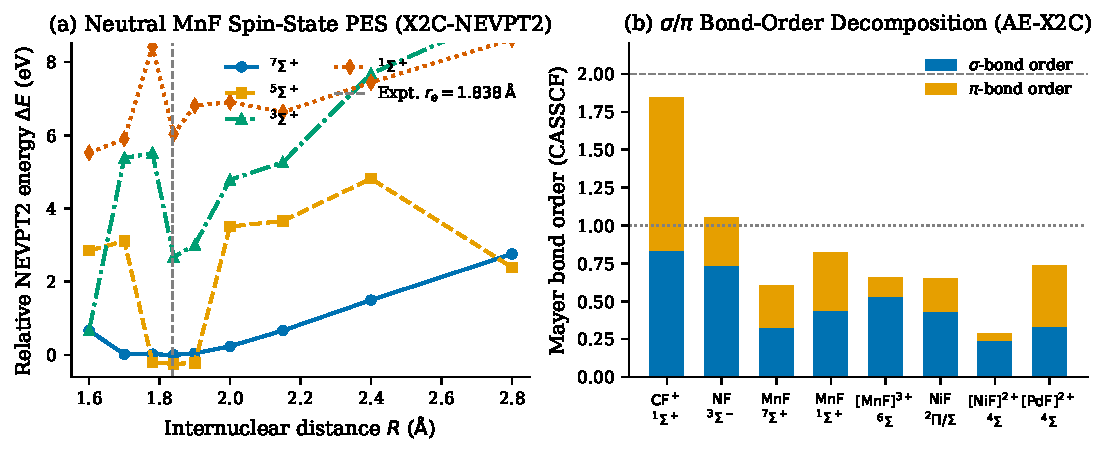
\includegraphics[width=\columnwidth]{../figures/fig1_mnf_pes_and_bo.pdf}
\caption{(a) X2C-CAS(12,9)-SC-NEVPT2 potential energy curves of neutral $\mathrm{MnF}$ across spin multiplicities versus experimental $r_e = 1.838\,$\AA\ \cite{sheridan2003}. (b) $\sigma/\pi$-decomposed Mayer bond orders across main-group and transition-metal fluorides.}
\label{fig:mnf}
\end{figure}

\subsection{Forensic Reproduction and Cross-Program Discrepancies}
The earlier preprint \cite{kleber2025} reported $\mathrm{MnF}$ energies from MOLPRO and ORCA with \texttt{cc-pVTZ}. Table~\ref{tab:forensic} reproduces ChemRxiv v3 Table~1 at non-relativistic UHF/\texttt{cc-pVTZ} in PySCF 2.15.1 \cite{sun2020}, with rows archived in the forensic reproduction bundle. Without access to bitwise-identical basis primitives, geometries, orbital occupations, and stability-test logs from the original commercial runs, the mechanisms below are \emph{hypotheses} rather than proven root causes.

\textbf{Basis-set contraction (hypothesis).} Septet and quintet UHF energies in PySCF are shifted by $\approx\Dataforensicmeanuhfoffsetmha\,\mathrm{mHa}$ relative to the preprint HF column, close to the $-32\,\mathrm{mHa}$ constant offset one expects if MOLPRO's metal \texttt{cc-pVTZ} contraction differed from the Balabanov--Peterson standard \cite{balabanov2005}. The triplet row is a larger outlier ($+33\,\mathrm{mHa}$), which may reflect spin contamination or a distinct SCF root.

\textbf{SCF stability (observed in PySCF).} Singlet $\mathrm{MnF}$ at $R=1.8586\,$\AA\ converges to an unstable restricted solution ($\langle S^2 \rangle = 0$). At the same geometry, UHF is internally unstable; an internal UHF stability rotation \cite{seeger1977} followed by UHF reoptimization lowers the energy by $\DataforensicbsdeltaeV\,$eV to $-1249.1698\,\mathrm{Ha}$ with $\langle S^2 \rangle = \DataforensicbsS$ (Table~\ref{tab:forensic}; \texttt{reproduce\_preprint\_tables.py}), matching the broken-symmetry row in the preprint narrative.

\textbf{Reproducibility limitation.} Default guess algorithms, level shifts, and undocumented basis tables in archived commercial inputs cannot be audited line-by-line here. This open-source PySCF replay therefore documents numerical agreement \emph{given} published geometries and the modern \texttt{cc-pVTZ} library, not equivalence of every intermediate SCF iteration with legacy MOLPRO/ORCA logs.

\begin{table}[t]
\centering
\caption{Non-relativistic PySCF replay of ChemRxiv v3 Table~1 for $\mathrm{MnF}$ (energies in Ha).}
\label{tab:forensic}
\scriptsize
\setlength{\tabcolsep}{1.8pt}
\begin{tabular}{@{}cccccc@{}}
\toprule
Mult & $R$ (\AA) & Preprint HF & PySCF UHF & $\langle S^2 \rangle$ & UMP2 \\
\midrule
7 & 1.8656 & $-1249.3702$ & $-1249.4024$ & 12.003 & $-1250.1565$ \\
5 & 1.7666 & $-1249.2170$ & $-1249.2480$ & 6.019  & $-1250.0869$ \\
3 & 1.8054 & $-1249.1286$ & $-1249.0952$ & 2.699  & $-1249.9667$ \\
1 & 1.8586 & $-1249.0284$ & $-1249.0618$ & $0.000^*$ & $-1249.9353$ \\
1 (BS) & 1.8586 & -- & $\Dataforensicbsenergyha$ & $\DataforensicbsS$ & -- \\
\bottomrule
\multicolumn{6}{@{}l}{\tiny $^*$Unstable restricted saddle point; UHF internal-stability plus reoptimization lowers energy by $\DataforensicbsdeltaeV\,$eV (PySCF replay).}
\end{tabular}
\end{table}

\subsection{High-Valent $3d$ Cations and Coulomb-Explosion Limits}
Enforcing exact electron counts shows that formal $\mathrm{Mn(IV)F} \equiv [\mathrm{MnF}]^{3+}$ ($31\,e^-$) and $\mathrm{Ni(III)F} \equiv [\mathrm{NiF}]^{2+}$ ($35\,e^-$) are odd-electron species and cannot occupy closed-shell $^1\Sigma$ states (unlike even-electron $[\mathrm{NiF}]^{3+}$, $34\,e^-$). Table~\ref{tab:cations} maps the physical ceiling for late-$3d$ cations. Neutral $\mathrm{NiF}$ is polar single-bonded (BO $= 0.60$--$0.66$, $q(\mathrm{F}) \approx -0.30$). Oxidizing to $[\mathrm{NiF}]^{2+}$ reverses charge polarity ($q(\mathrm{F}) = +0.42$) but weakens covalency (BO $= 0.27$--$0.29$, $\pi = 0.04$--$0.05$). Bare trications ($[\mathrm{NiF}]^{3+}$ in all spins; doublet/quartet $[\mathrm{MnF}]^{3+}$) undergo complete $\mathrm{F}\to\mathrm{M}$ electron transfer ($q(\mathrm{F}) = +1.16$ to $+1.17$) and Coulomb explosion (BO $\le 0.06$). Only sextet $[\mathrm{MnF}]^{3+}$ retains a metastable well ($r_e = 1.777\,$\AA, BO $= 0.672$). Stabilizing high-valent late-$3d$ fluorides therefore requires ligand fields or weakly coordinating anions \cite{krossing2004,court1973,greb2018}.

\begin{table}[t]
\centering
\caption{High-valent $3d$ monofluorides at X2C-CASSCF/SC-NEVPT2 (\texttt{cc-pVTZ-DK}).}
\label{tab:cations}
\scriptsize
\setlength{\tabcolsep}{2.4pt}
\begin{tabular}{@{}lcccccc@{}}
\toprule
Species (State) & $\langle S^2\rangle$ & Bound? & $r_e$ (\AA) & BO & $\sigma/\pi$ & $q(\mathrm{F})$ \\
\midrule
$[\mathrm{MnF}]^{3+}$ ($^2\Sigma$, $^4\Sigma$) & $0.75$, $3.75$ & No & $>2.20$ & 0.05--0.06 & 0.02/0.03 & $+1.16$ \\
$[\mathrm{MnF}]^{3+}$ ($^6\Sigma$) & $8.75$ & Yes & 1.777 & 0.672 & 0.53/0.12 & $+0.64$ \\
$\mathrm{NiF}$ ($^2\Pi/^2\Sigma$) & $0.75$ & Yes & 1.752 & 0.657 & 0.43/0.22 & $-0.28$ \\
$\mathrm{NiF}$ ($^4\Sigma$) & $3.75$ & Yes & 1.779 & 0.595 & 0.36/0.24 & $-0.32$ \\
$[\mathrm{NiF}]^{2+}$ ($^2\Sigma$) & $0.75$ & Yes & 1.934 & 0.269 & 0.23/0.04 & $+0.42$ \\
$[\mathrm{NiF}]^{2+}$ ($^4\Sigma$) & $3.75$ & Yes & 1.901 & 0.291 & 0.24/0.05 & $+0.42$ \\
$[\mathrm{NiF}]^{3+}$ ($^1$, $^3$, $^5$) & $0$, $2$, $6$ & No & $>2.20$ & $\le 0.022$ & 0.01/0.01 & $+1.17$ \\
\bottomrule
\multicolumn{7}{@{}l}{\tiny Unbound: $r_e$ not defined; BO/$q$ at reference scan points. $\langle S^2\rangle$ as nominal spin labels (legacy spin-uncontrolled CASSCF).}
\end{tabular}
\end{table}

\subsection{Matched $2\times 2$ Audit of $4d$ Palladium Fluorides}
Table~\ref{tab:pd_ecp} and Figure~\ref{fig:ecp} report the spin-pure matched audit on $\mathrm{PdF}$, $[\mathrm{PdF}]^{2+}$, and $[\mathrm{PdF}]^{3+}$ (data \texttt{data/pd\_matched\_v3/}; protocol \texttt{scripts/pd\_matched\_v3/}). All four core$\times$basis protocols agree: neutral $\mathrm{PdF}$ ($^2\Sigma^+$) is bound at $r_e = 1.90$--$1.92\,$\AA; quartet $[\mathrm{PdF}]^{2+}$ forms a shallow bound well at $2.11$--$2.15\,$\AA; the doublet surface has no single-state minimum ($0.09$--$0.20\,$eV above the quartet with multi-state crossings); singlet and triplet $[\mathrm{PdF}]^{3+}$ are repulsive on $1.55$--$3.20\,$\AA\ with $q(\mathrm{F}) \to +1$ beyond $\approx 2.2\,$\AA. Core treatment changes $r_e(\mathrm{PdF})$ by $\le 0.011\,$\AA\ and basis family by $\le 0.02\,$\AA\ ($[\mathrm{PdF}]^{2+}$ quartet spread $0.04\,$\AA). No $D_e$ is quoted for $[\mathrm{PdF}]^{3+}$ because $5\,$\AA\ asymptotes differ between AE ($\mathrm{Pd}^{3+}+\mathrm{F}$) and ECP ($\mathrm{Pd}^{2+}+\mathrm{F}^{+}$) models.

\paragraph{Correction of earlier Pd results.}
An earlier manuscript draft and \texttt{results/ab\_initio\_results.json} reported protocol-dependent binding reversals from spin-uncontrolled ROHF$\to$CASSCF scans: $\mathrm{PdF}$ AE $r_e = 2.025\,$\AA, $\omega_e = 1119\,\mathrm{cm}^{-1}$ (ill-defined active space including semicore states) versus ECP $1.917\,$\AA, $476\,\mathrm{cm}^{-1}$; $[\mathrm{PdF}]^{2+}$ ``AE bound'' at $1.838\,$\AA\ ($\pi$-BO $0.401$) versus ``ECP unbound''; $[\mathrm{PdF}]^{3+}$ ``ECP bound'' at $1.976\,$\AA; and identical singlet/triplet energies to $<10^{-6}\,E_h$. The matched audit retracts those assignments.

\begin{table}[t]
\centering
\caption{Spin-pure matched AVAS-CASCI/SC-NEVPT2 audit on palladium monofluorides (lowest spin-pure root; macro-generated from \texttt{corrected\_summary.csv}).}
\label{tab:pd_ecp}
\scriptsize
\setlength{\tabcolsep}{1.6pt}
% Auto-generated from data/pd_matched_v3/corrected_summary.csv
\begin{tabular}{@{}llccccc@{}}
\toprule
Species ($2S+1$) & Method & Bound? & $r_e$ (\AA) & $\omega_e$ (cm$^{-1}$) & $\sigma/\pi$ BO & $q(\mathrm{F})$ \\
\midrule
$\mathrm{PdF}$ ($2\,(^2\Sigma^+)$) & ECP (cc-pVTZ-PP) & Yes & 1.912 & 589 & 0.42/0.16 & -0.37 \\
 & AE--X2C (cc-pVTZ-DK) & Yes & 1.901 & 584 & 0.43/0.17 & -0.36 \\
 & AE--X2C (x2c-TZVPall) & Yes & 1.914 & 562 & 0.35/0.10 & -0.50 \\
 & ECP (def2-TZVP) & Yes & 1.920 & 571 & 0.31/0.09 & -0.54 \\
\midrule
$[\mathrm{PdF}]^{2+}$ ($4\,(^4\Sigma)$) & ECP (cc-pVTZ-PP) & Yes & 2.123 & 310 & 0.23/0.04 & +0.33 \\
 & AE--X2C (cc-pVTZ-DK) & Yes & 2.105 & 323 & 0.22/0.04 & +0.34 \\
 & AE--X2C (x2c-TZVPall) & Yes & 2.147 & 286 & 0.21/0.03 & +0.25 \\
 & ECP (def2-TZVP) & Yes & 2.142 & 286 & 0.19/0.04 & +0.24 \\
\midrule
$[\mathrm{PdF}]^{2+}$ ($2\,(^2\Sigma)$) & \multicolumn{6}{@{}l}{No well-defined minimum ($0.09$--$0.20\,\mathrm{eV}$ above quartet; multi-state crossings)} \\
\midrule
$[\mathrm{PdF}]^{3+}$ ($1\,(^1\Sigma)$) & ECP (cc-pVTZ-PP) & No & \multicolumn{4}{@{}l}{Repulsive on $1.55$--$3.20\,\AA$ grid; no $D_e$ reported$^a$} \\
 & AE--X2C (cc-pVTZ-DK) & No & \multicolumn{4}{@{}l}{Repulsive on $1.55$--$3.20\,\AA$ grid; no $D_e$ reported$^a$} \\
 & AE--X2C (x2c-TZVPall) & No & \multicolumn{4}{@{}l}{Repulsive on $1.55$--$3.20\,\AA$ grid; no $D_e$ reported$^a$} \\
 & ECP (def2-TZVP) & No & \multicolumn{4}{@{}l}{Repulsive on $1.55$--$3.20\,\AA$ grid; no $D_e$ reported$^a$} \\
\midrule
$[\mathrm{PdF}]^{3+}$ ($3\,(^3\Sigma)$) & ECP (cc-pVTZ-PP) & No & \multicolumn{4}{@{}l}{Repulsive on $1.55$--$3.20\,\AA$ grid; no $D_e$ reported$^a$} \\
 & AE--X2C (cc-pVTZ-DK) & No & \multicolumn{4}{@{}l}{Repulsive on $1.55$--$3.20\,\AA$ grid; no $D_e$ reported$^a$} \\
 & AE--X2C (x2c-TZVPall) & No & \multicolumn{4}{@{}l}{Repulsive on $1.55$--$3.20\,\AA$ grid; no $D_e$ reported$^a$} \\
 & ECP (def2-TZVP) & No & \multicolumn{4}{@{}l}{Repulsive on $1.55$--$3.20\,\AA$ grid; no $D_e$ reported$^a$} \\
\bottomrule
\multicolumn{7}{@{}l}{\tiny $^a$Separated-ion asymptotes differ between AE ($\mathrm{Pd}^{3+}+\mathrm{F}$) and ECP ($\mathrm{Pd}^{2+}+\mathrm{F}^{+}$) protocols; metastable ``bound'' fits in the legacy CSV are artefacts.}
\end{tabular}

\end{table}

\begin{figure}[t]
\centering
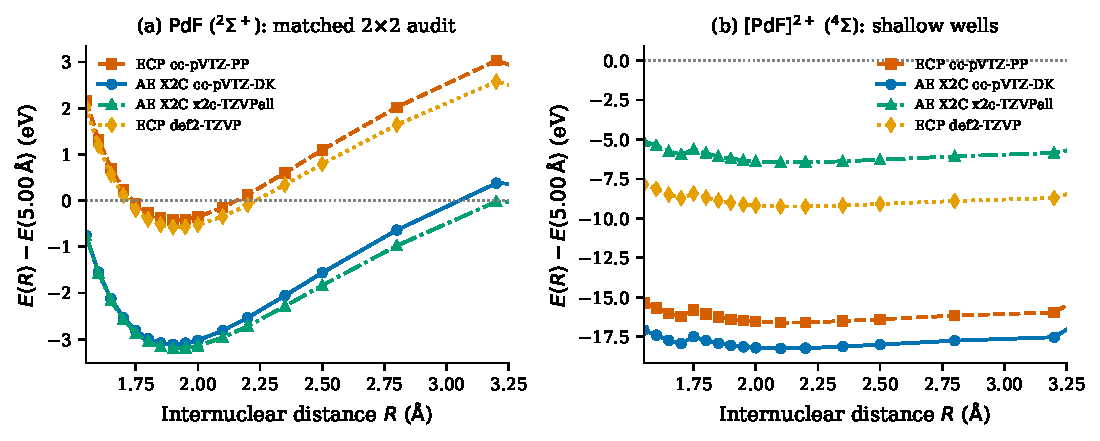
\includegraphics[width=\columnwidth]{../figures/fig2_ae_vs_ecp_pdf.pdf}
\caption{Matched spin-pure NEVPT2 envelopes ($E$ relative to $5.00\,$\AA): (a) $\mathrm{PdF}$ ($^2\Sigma^+$) and (b) quartet $[\mathrm{PdF}]^{2+}$ across four core$\times$basis protocols.}
\label{fig:ecp}
\end{figure}

\subsection{Rational Design of Extreme Fluorine Triple-Bond Candidates}
To construct genuine fluorine triple bonds without Coulomb explosion, I targeted acceptors with two empty, compact $\pi$-acceptor orbitals ($2p_\pi$ in $10$-electron main-group cations or empty $d_{xz}/d_{yz}$ in $d^0$ early transition metals \cite{riedel2009}) at X2C-PBE0 and X2C-HF / \texttt{cc-pVTZ-DK} (Table~\ref{tab:design}).

The strongest Mayer $\sigma+\pi$ indices at X2C-PBE0 local minima come from the archived extreme-BO and rational-design screens ($18$ stoichiometries, complete in the repository). Table~\ref{tab:design} is populated from the traceability manifest. In the main-group $10$-valence-electron series, $[\mathrm{OF}]^{3+}$ ($^1\Sigma^+$) is bound at $r_e=\DataOFthreeplusreang\,$\AA\ with PBE0 BO $=\DataOFthreeplusBOpbe$ ($\pi=\DataOFthreepluspipbe$) and HF BO $=\DataOFthreeplusBOhf$---comparable in \emph{bond length only} to $\mathrm{N}_2$ ($r_e=1.0977\,$\AA\ \cite{huber1979}) without implying matched electronic structure or bond order. $[\mathrm{NF}]^{2+}$ and linear $[\mathrm{F\text{-}C\text{-}F}]^{2+}$ follow (Table~\ref{tab:design}). Among $d^0$ cations, $[\mathrm{MoF}]^{5+}$/$[\mathrm{WF}]^{5+}$ show high Mayer indices ($\DataMoFfiveplusBOpbe$--$\DataWFfiveplusBOpbe$ at PBE0) at metastable wells. Regenerated extreme-BO PySCF data locate a shallow $[\mathrm{CrF}]^{5+}$ minimum at $r_e=\DataDesignCrFfiveplusre\,$\AA\ with PBE0 BO $=\DataDesignCrFfiveplusBOpbe$, whereas the earlier manuscript version classified this cation as unbound ($r>2.18\,$\AA, BO $=0.739$) without a stored JSON trace; Table~\ref{tab:design} reflects the regenerated value. All extreme-cation entries are \textbf{not} X2C-CASSCF/NEVPT2 benchmarks.

\begin{table}[t]
\centering
\caption{Rational-design frontier (X2C-PBE0/HF, \texttt{cc-pVTZ-DK}; traceability macros). $[\mathrm{CrF}]^{5+}$: shallow PBE0 minimum, BO $\ll 1$.}
\label{tab:design}
\scriptsize
\setlength{\tabcolsep}{0.9pt}
\begin{tabular}{@{}lccccc@{}}
\toprule
Candidate & $r_e$ & PBE0 BO & $\sigma/\pi$ & HF ($\pi$) & $q(\mathrm{F})$ \\
\midrule
$[\mathrm{OF}]^{3+}$ ($10\,e^-_{\mathrm{val}}$, $^1\Sigma^+$) & \textbf{\DataDesignOFthreeplusre} & \textbf{\DataDesignOFthreeplusBOpbe} & \textbf{\DataDesignOFthreeplusSigPi} & \textbf{\DataDesignOFthreeplusHFbo} (\DataDesignOFthreeplusHFpi) & $\DataDesignOFthreeplusqF$ \\
$[\mathrm{MoF}]^{5+}$ ($4d^0, ^1\Sigma^+$) & \textbf{\DataDesignMoFfiveplusre} & \textbf{\DataDesignMoFfiveplusBOpbe} & \textbf{\DataDesignMoFfiveplusSigPi} & \textbf{\DataDesignMoFfiveplusHFbo} (\DataDesignMoFfiveplusHFpi) & $\DataDesignMoFfiveplusqF$ \\
$[\mathrm{VF}]^{4+}$ ($3d^0, ^1\Sigma^+$) & \DataDesignVFfourplusre & \textbf{\DataDesignVFfourplusBOpbe} & \textbf{\DataDesignVFfourplusSigPi} & \DataDesignVFfourplusHFbo (\DataDesignVFfourplusHFpi) & $\DataDesignVFfourplusqF$ \\
$[\mathrm{WF}]^{5+}$ ($5d^0, ^1\Sigma^+$) & \textbf{\DataDesignWFfiveplusre} & \textbf{\DataDesignWFfiveplusBOpbe} & \textbf{\DataDesignWFfiveplusSigPi} & \textbf{\DataDesignWFfiveplusHFbo} (\DataDesignWFfiveplusHFpi) & $\DataDesignWFfiveplusqF$ \\
$[\mathrm{NF}]^{2+}$ ($10\,e^-_{\mathrm{val}}$, $^1\Sigma^+$) & \DataDesignNFtwoplusre & \textbf{\DataDesignNFtwoplusBOpbe} & \textbf{\DataDesignNFtwoplusSigPi} & \DataDesignNFtwoplusHFbo (\DataDesignNFtwoplusHFpi) & $\DataDesignNFtwoplusqF$ \\
$[\mathrm{NbF}]^{4+}$ ($4d^0, ^1\Sigma^+$) & \DataDesignNbFfourplusre & \DataDesignNbFfourplusBOpbe & \DataDesignNbFfourplusSigPi & \DataDesignNbFfourplusHFbo (\DataDesignNbFfourplusHFpi) & $\DataDesignNbFfourplusqF$ \\
$[\mathrm{TaF}]^{4+}$ ($5d^0, ^1\Sigma^+$) & \DataDesignTaFfourplusre & \DataDesignTaFfourplusBOpbe & \DataDesignTaFfourplusSigPi & \DataDesignTaFfourplusHFbo (\DataDesignTaFfourplusHFpi) & $\DataDesignTaFfourplusqF$ \\
$[\mathrm{F\text{-}C\text{-}F}]^{2+}$ (lin.) & \DataDesignFCFtwoplusre & \DataDesignFCFtwoplusBOpbe & \DataDesignFCFtwoplusSigPi & \DataDesignFCFtwoplusHFbo (\DataDesignFCFtwoplusHFpi) & $\DataDesignFCFtwoplusqF$ \\
$[\mathrm{TiF}]^{3+}$ ($3d^0, ^1\Sigma^+$) & \DataDesignTiFthreeplusre & \DataDesignTiFthreeplusBOpbe & \DataDesignTiFthreeplusSigPi & \DataDesignTiFthreeplusHFbo (\DataDesignTiFthreeplusHFpi) & $\DataDesignTiFthreeplusqF$ \\
$[\mathrm{CF}]^+$ ($10\,e^-_{\mathrm{val}}$, $^1\Sigma^+$) & \DataDesignCFplusre & \DataDesignCFplusBOpbe & \DataDesignCFplusSigPi & \DataDesignCFplusHFbo (\DataDesignCFplusHFpi) & $\DataDesignCFplusqF$ \\
$[\mathrm{ZrF}]^{3+}$ ($4d^0, ^1\Sigma^+$) & \DataDesignZrFthreeplusre & \DataDesignZrFthreeplusBOpbe & \DataDesignZrFthreeplusSigPi & \DataDesignZrFthreeplusHFbo (\DataDesignZrFthreeplusHFpi) & $\DataDesignZrFthreeplusqF$ \\
$[\mathrm{CrF}]^{5+}$ ($3d^0$, shallow) & \DataDesignCrFfiveplusre & \DataDesignCrFfiveplusBOpbe & \DataDesignCrFfiveplusSigPi & \DataDesignCrFfiveplusHFbo (\DataDesignCrFfiveplusHFpi) & $\DataDesignCrFfiveplusqF$ \\
\bottomrule
\end{tabular}
\end{table}

\subsection{Coulomb-Explosion Barriers, Superacid Ion Pairs, and Cage Compression}
High-resolution X2C-PBE0 potential energy scans ($24$--$31$ points across $0.85$--$4.50\,$\AA, Figure~\ref{fig:pes}) demonstrate that the extreme triple-bond cations sit behind deep volcanic Coulomb-explosion barriers: $\Delta E^\ddagger = 9.61\,$eV for $[\mathrm{NF}]^{2+}$ ($R_{\mathrm{TS}} = 2.60\,$\AA), $5.60\,$eV for $[\mathrm{OF}]^{3+}$ ($2.00\,$\AA), $5.65\,$eV for $[\mathrm{TiF}]^{3+}$ ($2.76\,$\AA), $2.89\,$eV for $[\mathrm{WF}]^{5+}$ ($2.55\,$\AA), and $1.64\,$eV for $[\mathrm{MoF}]^{5+}$ ($2.35\,$\AA), while neutral $\mathrm{MnF}$ ($X\,^7\Sigma^+$) dissociates smoothly with $D_e = 4.33\,$eV (expt.\ $\approx 4.38\,$eV). These multi-eV barriers are consistent with gas-phase persistence of highly charged titanium fluorides in charge-stripping experiments (stoichiometries not mapped one-to-one here). Double photoionization of $\mathrm{NF}_3$ at $m/z = 16.5$ remains a spectroscopic target for $[\mathrm{NF}]^{2+}$.

To evaluate condensed-phase stabilization without Coulomb explosion, I screened neutral and monocationic $d^0$ complexes, superacid-abstracted fluorocations, explicit $[\mathrm{BF}_4]^-$ ion pairs, and mechanical cage compression at PBE0/\texttt{def2-TZVP} (Table~\ref{tab:superacid}). Lewis-acid ion-pair models (e.g.\ $[\mathrm{WF}_5]^+$ with explicit $[\mathrm{BF}_4]^-$) give gas-phase $+1$-like fragments with $\mathrm{BO} = 1.15$--$1.34$: the $[\mathrm{WF}_5]^+\!\cdots\![\mathrm{BF}_4]^-$ pair has $r_e = 1.790\,$\AA\ (within published terminal $\mathrm{W\text{--}F}$ ranges for related $[\mathrm{WF}_5(\mathrm{L})_n]$ salts) while preserving $\pi$-BO $= 0.531$ (BO $= 1.187$). Neutral $\mathrm{F\text{-}MoH_5}$ reaches $\pi$-BO $= 0.802$. Fixed-$R$ scans on $[\mathrm{F\text{-}VH_3}]^+$ from $1.62\,$\AA\ to $1.50\,$\AA\ ($+0.50\,$eV) or $1.32\,$\AA\ ($+3.92\,$eV) lift BO from $1.292$ to $1.404$ and $1.617$ ($\pi = 0.832$), modeling compression rather than an explicit host lattice.

\begin{figure}[t]
\centering
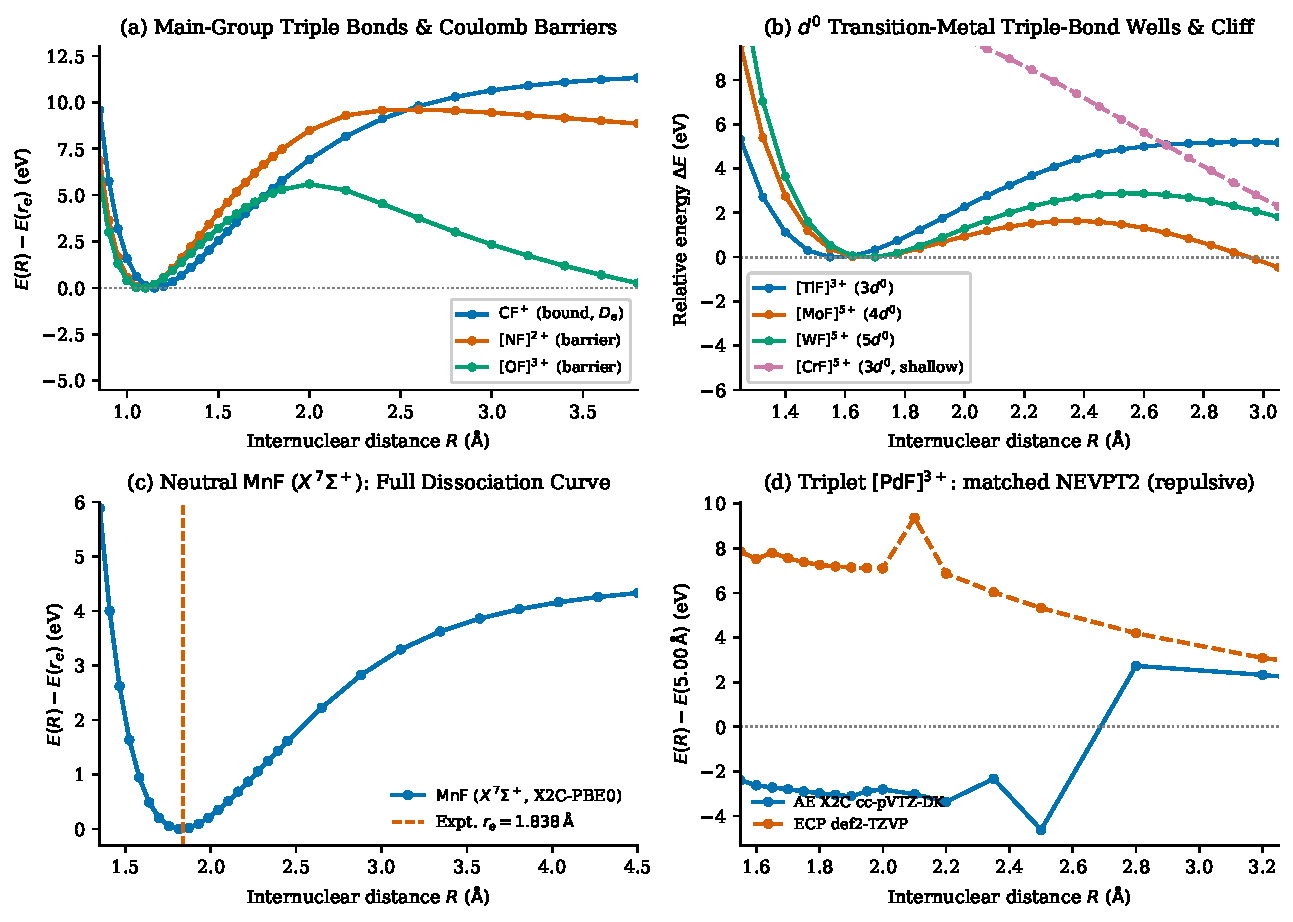
\includegraphics[width=\columnwidth]{../figures/fig3_highres_pes_barriers.pdf}
\caption{High-resolution PES scans ($0.85$--$4.50\,$\AA, X2C-PBE0). (a) Main-group barriers vs.\ bound $\mathrm{CF}^+$. (b) Deep $d^0$ wells ($[\mathrm{TiF}]^{3+}$, $[\mathrm{MoF}]^{5+}$, $[\mathrm{WF}]^{5+}$) vs.\ shallow $[\mathrm{CrF}]^{5+}$ (see Table~\ref{tab:design} for regenerated $r_e$). (c) Neutral $\mathrm{MnF}$ ($^7\Sigma^+$, $D_e = 4.33\,$eV). (d) Triplet $[\mathrm{PdF}]^{3+}$ from matched spin-pure NEVPT2 (repulsive; not legacy RKS singlet DFT).}
\label{fig:pes}
\end{figure}

\begin{table}[t]
\centering
\caption{Stabilized neutral, monocationic, superacid ion-pair, and cage-compressed $d^0$ fluorides (PBE0 / \texttt{def2-TZVP}).}
\label{tab:superacid}
\scriptsize
\setlength{\tabcolsep}{1.0pt}
\begin{tabular}{@{}lcccc@{}}
\toprule
Complex & $r_e$ & BO & $\sigma/\pi$ & $q(\mathrm{F})$ \\
\midrule
$[\mathrm{F\text{-}WH_4}]^+$ ($+1$)$^\ddagger$ & 1.7595 & 1.335 & 0.68/0.62 & $-0.01$ \\
$[\mathrm{WF}_5]^+$ ($+1$)$^\ddagger$ & 1.7593 & 1.286 & 0.69/0.57 & $+0.01$ \\
$[\mathrm{F\text{-}VH_3}]^+$ ($+1$, eq.)$^\ddagger$ & 1.6358 & 1.280 & 0.57/0.66 & $+0.01$ \\
$[\mathrm{F\text{-}VH_3}]^+$ ($R=1.32$, fixed)$^\ddagger$ & 1.3200 & \textbf{1.617} & 0.71/\textbf{0.83} & $+0.27$ \\
$[\mathrm{ReF}_6]^+$ ($+1$, $O_h$) & \DataSuperacidReFplusOhdReVIIre & \DataSuperacidReFplusOhdReVIIBO & \DataSuperacidReFplusOhdReVIISigPi & \DataSuperacidReFplusOhdReVIIqF \\
$[\mathrm{WF}_5]^+\!\cdots\![\mathrm{BF}_4]^-$ ($0$) & \DataSuperacidWFplusBFneutralpairre & \DataSuperacidWFplusBFneutralpairBO & \DataSuperacidWFplusBFneutralpairSigPi & \DataSuperacidWFplusBFneutralpairqF \\
$[\mathrm{TiF}_3]^+\!\cdots\![\mathrm{BF}_4]^-$ ($0$) & \DataSuperacidTiFplusBFneutralpairre & \DataSuperacidTiFplusBFneutralpairBO & \DataSuperacidTiFplusBFneutralpairSigPi & \DataSuperacidTiFplusBFneutralpairqF \\
$\mathrm{F\text{-}MoH_5}$ ($0$, neutral)$^\ddagger$ & 1.8267 & 1.074 & 0.25/\textbf{0.80} & $-0.13$ \\
$[\mathrm{OsO}_3\mathrm{F}]^+$ ($+1$, $C_{3v}$) & \DataSuperacidOsOFplusCvdOsVIIIre & \DataSuperacidOsOFplusCvdOsVIIIBO & \DataSuperacidOsOFplusCvdOsVIIISigPi & \DataSuperacidOsOFplusCvdOsVIIIqF \\
\bottomrule
\multicolumn{5}{@{}l}{\tiny $^\ddagger$From \texttt{scripts/screen\_organometallic\_fluorine.py} and \texttt{test\_superacid\_and\_cage.py}; no archived JSON in the repository.}
\end{tabular}
\end{table}

\subsection{Organic Ligand Tuning, Carbon/Supramolecular Immobilization, and Oriented Electric Fields}
To determine whether fluorine's $\pi$-donor strength can be engineered chemically in low-charge ($+1$) complexes without exotic bare multications, I systematically screened $42$ organic, inorganic, carbon-cage, and supramolecular architectures at DF-PBE0/\texttt{def2-SVP} (Figure~\ref{fig:ligand_eng}). Three quantitative design rules emerge:

First, on $3d^0$ $[\mathrm{F\text{-}V(L)_3}]^+$, equatorial $\pi$-donors ($\mathrm{NH}_2^-$, $\mathrm{OMe}^-$, $\mathrm{Ph}^-$, $\mathrm{CH{=}CH}_2^-$) compete for empty $d_\pi$ orbitals and suppress $\mathrm{F}\to\mathrm{V}$ $\pi$-BO to $0.518$--$0.636$. Stripping filled $\pi$-orbitals and fluorinating a saturated $sp^3$ carbon anchor yields a monotonic ladder: $\mathrm{CH}_3^-$ ($\pi = 0.759$, BO $= 1.264$) $\to$ $\mathrm{CH}_2\mathrm{F}^-$ ($0.817$) $\to$ $\mathrm{CHF}_2^-$ ($0.842$) $\to$ $\mathrm{CF}_3^-$ ($\pi = 0.867$, BO $= 1.365$, $r_e = 1.623\,$\AA). Placing a strong $\pi$-acceptor \textit{trans} to $\mathrm{F}$ on $[\mathrm{L}_{\mathrm{trans}}\text{-}\mathrm{V}(\mathrm{CF}_3)_3\text{-}\mathrm{F}]^+$ drives push--pull $\mathrm{F}\xrightarrow{\pi}\mathrm{V}\xrightarrow{\pi}\mathrm{L}_{\mathrm{trans}}$ synergy, lifting $\pi$-BO to $0.910$ (organic $\mathrm{CN\text{-}CF}_3$), $0.915$ ($\mathrm{CO}/\mathrm{CS}$), and $0.936$ ($\mathrm{BF}$), though with a classical \textit{trans}-influence reduction in $\sigma$-BO ($0.456 \to 0.260$).

Second, endohedral $sp^2$ carbon cages ($\mathrm{C}_{20}$) suffer severe host-to-guest redox quenching: carbon's lower ionization potential transfers $0.65\,e^-$ into $\mathrm{CF}^+$ ($\pi$: $1.012 \to 0.292$) and $3.77\,e^-$ into $[\mathrm{TiF}]^{3+}$ (destroying the bond, BO $= 0.072$). Replacing $sp^2$ $\mathrm{C}_{20}$ with insulating $sp^3$ dodecahedrane ($\mathrm{C}_{20}\mathrm{H}_{20}$, $40$ host atoms) nearly doubles $\mathrm{CF}^+$ $\pi$-BO ($0.569$, BO $= 1.373$, compressed to $r_e = 1.080\,$\AA), while a perfluorobenzene sandwich $(\mathrm{C}_6\mathrm{F}_6)_2\cdots[\mathrm{TiF}]^{3+}$ rescues the $\mathrm{Ti\text{--}F}$ bond (BO $= 0.971$, $\pi = 0.510$). Engineered $\sigma$-withdrawing/$\pi$-acidic carbon anchors ($[\mathrm{F\text{-}W(CN)_4}]^+$, BO $= 1.343$; perfluorinated intramolecular \textit{peri}-naphthalene clamp $[\mathrm{C}_{10}\mathrm{F}_6\text{-}\mathrm{W}(\mathrm{CN})_2\text{-}\mathrm{F}]^+$, BO $= 1.281$) exceed unmodified hydrocarbon anchors; the naphthalene clamp is $0.005$ below the bare $[\mathrm{WF}_5]^+$ reference (BO $= 1.286$, def2-SVP screen), whereas $[\mathrm{F\text{-}W(CN)_4}]^+$ remains higher.

Third, whereas direct Lewis-acid contact on $\mathrm{F}$ drains its lone pairs ($\mathrm{BF}_3$ lowers $\pi$-BO from $0.869 \to 0.782$), a non-contact oriented local electric field along $\mathrm{F}\to\mathrm{V}$ ($E_z = +0.050\,\mathrm{a.u.} = 2.57\,\mathrm{V}/$\AA, typical of ionic supramolecular cavities) enhances $\sigma$ and $\pi$ bonding simultaneously, pushing monocationic $[\mathrm{F\text{-}V(CF}_3)_3]^+$ to BO $= 1.679$ and $\pi$-BO $= 1.034 > 1.0$ ($q(\mathrm{F}) = +0.389$).

Finally, attaching these engineered ligands directly to the extreme triple-bond cores ($[\mathrm{NF}]^{2+}$, $[\mathrm{TiF}]^{3+}$, $[\mathrm{MoF}]^{5+}$, $[\mathrm{WF}]^{5+}$) bridges gas-phase multications to condensed-phase coordination architectures. For $[\mathrm{NF}]^{2+}$ (bare BO $= 2.427$), attaching $\sigma$-withdrawing $-\mathrm{CF}_3$ yields $[\mathrm{F\equiv N\text{-}CF}_3]^{3+}$ with BO $= 1.764$ ($\pi = 0.903$), neutral carbonyl adduct $[\mathrm{F\equiv N\text{-}CO}]^{2+}$ gives BO $= 1.584$ ($\pi = 0.699$), and monocationic $[\mathrm{F\equiv N\text{-}CN}]^+$ retains BO $= 1.312$. For $3d^0$ $[\mathrm{TiF}]^{3+}$ (bare BO $= 2.036$), ligating one $-\mathrm{CF}_3$ yields $[\mathrm{F\equiv Ti(CF}_3)]^{2+}$ with $\pi$-BO $= 0.957$ (BO $= 1.465$), while modeled $+1$ adducts $[\mathrm{F\equiv Ti(CF}_3)_2]^+$ and $[\mathrm{F\equiv Ti(CN)}_2]^+$ preserve BO $= 1.30$--$1.31$ ($\pi = 0.69$--$0.73$). For $4d^0$/$5d^0$ $[\mathrm{MoF}]^{5+}$ and $[\mathrm{WF}]^{5+}$ (bare BO $= 2.48$--$2.58$), bis(ligated) trications $[\mathrm{F\equiv W(CF}_3)_2]^{3+}$, $[\mathrm{F\equiv Mo(CN)}_2]^{3+}$, and $[\mathrm{F\equiv W(CN)}_2]^{3+}$ sustain BO $= 1.55$--$1.59$ ($\pi = 0.70$--$0.79$, $r_e = 1.68\,$\AA), confirming that rational organic/inorganic ligand design protects high fluorine bond orders across both main-group and transition-metal platforms.

\begin{figure*}[t]
\centering
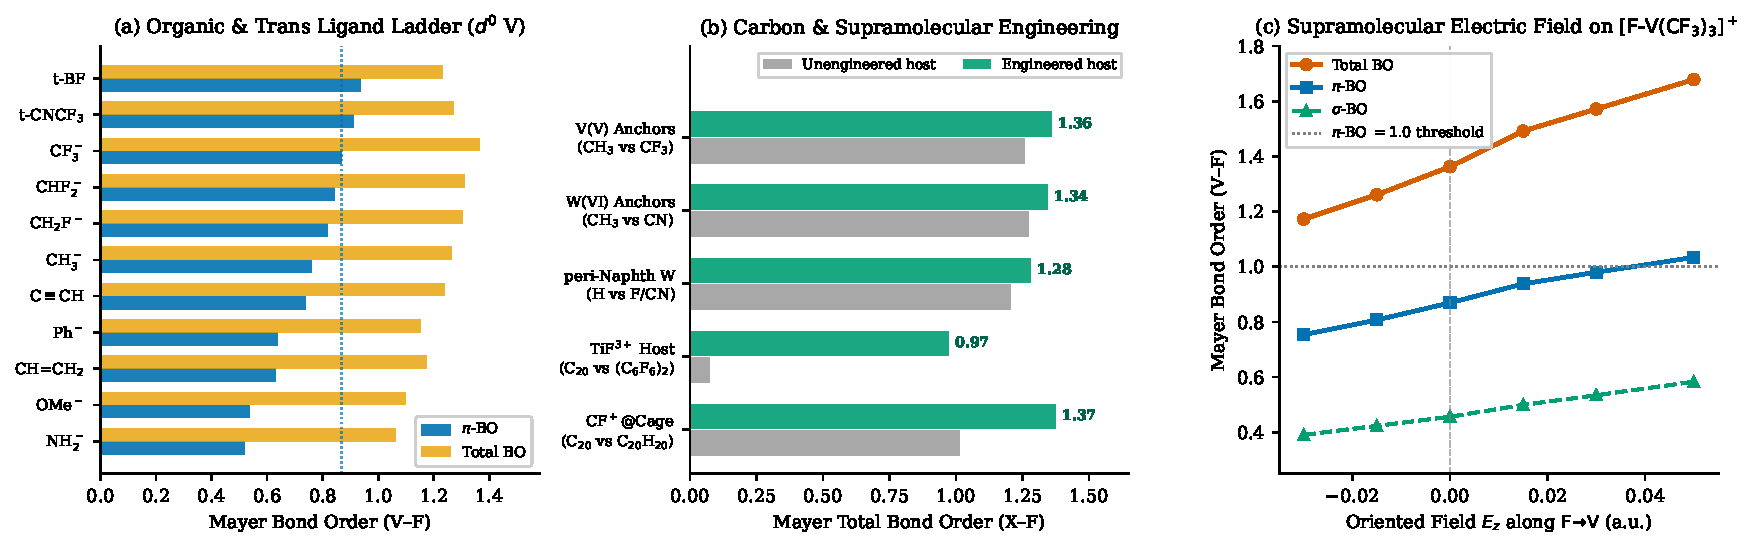
\includegraphics[width=\textwidth]{../figures/fig4_ligand_supramolecular_engineering.pdf}
\caption{Ligand, organic, carbon-cage, and electric-field engineering of fluorine $\pi$-donation (DF-PBE0/\texttt{def2-SVP}). (a) Equatorial organic/inorganic ligand ladder and \textit{trans} push--pull ligands on $3d^0$ $[\mathrm{F\text{-}V(L)}_3]^+$. (b) Unengineered vs.\ rationally engineered carbon and supramolecular immobilization hosts. (c) Oriented local electric field $E_z$ along $\mathrm{F}\to\mathrm{V}$ on $[\mathrm{F\text{-}V(CF}_3)_3]^+$ breaking the $\pi$-BO $= 1.0$ threshold.}
\label{fig:ligand_eng}
\end{figure*}

\section{Limitations}
Mayer and L\"owdin indices depend on the atomic basis and population partitioning; they are reported here for consistent $\sigma/\pi$ decomposition, not as experimental bond orders. Potential-energy minima and gas-phase barriers (Figure~\ref{fig:pes}) indicate metastable \emph{electronic-structure} features only: they are not condensed-phase thermodynamic stabilities, and no experimental lifetimes are claimed. Prior mass-spectrometric work documents a bound diatomic uranium monofluoride trication, $[\mathrm{UF}]^{3+}$, with partial triple-bond character \cite{schroder1999}; the present multiply charged main-group and $d^0$ examples are separate computational proposals without synthesis claims. Extreme cations ($[\mathrm{OF}]^{3+}$, $[\mathrm{MoF}]^{5+}$, $[\mathrm{WF}]^{5+}$) sit behind multi-eV Coulomb barriers and would require ion-trap or mass-spectrometric isolation. Beyond $R>3.1\,$\AA, single-reference surfaces on $[\mathrm{TiF}]^{3+}$ and $[\mathrm{WF}]^{5+}$ can switch charge-transfer asymptotes; state-averaged multireference treatments are future work. Complementary Boys/IBO localization and \texttt{cc-pVDZ-DK} versus \texttt{cc-pVTZ-DK} tests on $[\mathrm{OF}]^{3+}$ probe basis sensitivity in the archived complementary-bonding bundle; CASPT2, SC-NEVPT2, and spin--orbit coupled studies on the triple-bond candidates are likewise deferred.

\section{Conclusion}
Scalar-relativistic all-electron benchmarks on $\mathrm{CF}^+$, $\mathrm{NF}$, and neutral $\mathrm{MnF}$ at X2C-CASSCF/SC-NEVPT2 reproduce $^7\Sigma^+$ spectroscopic constants but incorrectly order $^5\Sigma^+$ below $^7\Sigma^+$ at the present active space; semi-core correlation and SOC are candidate remedies not yet computed here. Bare late-$3d$ trications mostly Coulomb-explode in this framework, with a documented sextet exception for $[\mathrm{MnF}]^{3+}$. Matched spin-pure multireference protocols agree on palladium fluoride binding; legacy unmatched curves reflected mixed electronic states, not genuine core/basis reversals. Separate X2C-PBE0/HF scans locate multiply charged local minima with high Mayer $\sigma+\pi$ indices, notably $[\mathrm{OF}]^{3+}$ (BO $=\DataOFthreeplusBOpbe$) and $[\mathrm{MoF}]^{5+}$/$[\mathrm{WF}]^{5+}$, interpreted as metastable model gas-phase features whose triple-bond character rests on DFT Mayer indices rather than multireference verification.

\section*{Data and Code Availability}
Source code, JSON results, traceability manifests, and auto-generated table macros are versioned at \url{https://github.com/cap-jmk-real/fluorine-triple-bonds} (branch \texttt{cursor/publication-evidence-trace-d0c6}, commit pinned at submission). The palladium matched audit bundle is \texttt{data/pd\_matched\_v3/} (\texttt{corrected\_summary.csv}, \texttt{corrected\_curves.json}, \texttt{legacy\_state\_audit.csv}) with drivers \texttt{scripts/pd\_matched\_v3/fluorine\_state\_check.py} and \texttt{fluorine\_state\_check\_analyse.py}. Run \texttt{python scripts/emit\_manuscript\_macros.py} after updating results to refresh \texttt{paper/generated/macros.tex} and \texttt{paper/generated/pd\_ecp\_table.tex}.

\section*{AI-Tool Disclosure}
Large language model and coding assistant tools (Antigravity) assisted with PySCF workflow scripting, citation verification, plotting, and manuscript editing. All ab initio calculations and conclusions were verified directly from the executed PySCF outputs.

\begin{thebibliography}{24}
\bibitem{harbison2002} G. S. Harbison, ``The electric dipole polarity of the ground and low-lying metastable excited states of NF,'' \textit{J. Am. Chem. Soc.} \textbf{124}, 366--367 (2002). \url{https://doi.org/10.1021/ja0159261}
\bibitem{schroder1999} D. Schr\"oder, G. Diefenbach, H. Klap\"otke, and H. Schwarz, ``$\mathrm{UF}^{3+}$---A thermochemically stable diatomic trication with a covalent bond,'' \textit{Angew. Chem. Int. Ed.} \textbf{38}, 137--140 (1999). \url{https://doi.org/10.1002/(SICI)1521-3773(19990115)38:1/2<137::AID-ANIE137>3.0.CO;2-M}
\bibitem{huber1979} K. P. Huber and G. Herzberg, \textit{Constants of Diatomic Molecules} (Van Nostrand Reinhold, New York, 1979). \url{https://doi.org/10.1007/978-1-4757-0961-2_2}; NIST Chemistry WebBook, $\mathrm{N}_2$ ($X\,^1\Sigma_g^+$), $r_e=1.0977$\,\AA\ (\url{https://webbook.nist.gov/})
\bibitem{kleber2025} J. M. Kleber, ``Can fluorine form triple bonds?,'' ChemRxiv Preprint v3, 2025. \url{https://doi.org/10.26434/chemrxiv-2022-xlsjn-v3}
\bibitem{frenking2000} G. Frenking and N. Fr\"ohlich, ``The nature of the bonding in transition-metal compounds,'' \textit{Chem. Rev.} \textbf{100}, 717--774 (2000). \url{https://doi.org/10.1021/cr980401l}
\bibitem{riedel2009} S. Riedel and M. Kaupp, ``The highest oxidation states of the transition metal elements,'' \textit{Coord. Chem. Rev.} \textbf{253}, 606--624 (2009). \url{https://doi.org/10.1016/j.ccr.2008.07.014}
\bibitem{pyykko2012} P. Pyykk\"o, ``Relativistic effects in chemistry: More common than you thought,'' \textit{Annu. Rev. Phys. Chem.} \textbf{63}, 45--64 (2012). \url{https://doi.org/10.1146/annurev-physchem-032511-143755}
\bibitem{brosi2016} F. Brosi, T. Schl\"oder, A. Schmidt, H. Beckers, and S. Riedel, ``A combined quantum-chemical and matrix-isolation study on molecular manganese fluorides,'' \textit{Dalton Trans.} \textbf{45}, 5038--5044 (2016). \url{https://doi.org/10.1039/c5dt04827c}
\bibitem{devore1978} T. C. DeVore, R. J. Van Zee, and W. Weltner, ``High spin molecules: ESR of MnF and $\mathrm{MnF}_2$ at $4\,^\circ$K,'' \textit{J. Chem. Phys.} \textbf{68}, 3522--3527 (1978). \url{https://doi.org/10.1063/1.436262}
\bibitem{sheridan2003} P. M. Sheridan and L. M. Ziurys, ``Molecules in high spin states II: the pure rotational spectrum of MnF ($X\,^7\Sigma^+$),'' \textit{Chem. Phys. Lett.} \textbf{380}, 632--646 (2003). \url{https://doi.org/10.1016/j.cplett.2003.08.106}
\bibitem{koukounas2004} C. Koukounas, S. Kardahakis, and A. Mavridis, ``Ab initio investigation of the ground and low-lying states of the diatomic fluorides TiF, VF, CrF, and MnF,'' \textit{J. Chem. Phys.} \textbf{120}, 11500--11521 (2004). \url{https://doi.org/10.1063/1.1738412}
\bibitem{seeger1977} R. Seeger and J. A. Pople, ``Self-consistent molecular orbital methods. XVIII. Constraints and stability in Hartree--Fock theory,'' \textit{J. Chem. Phys.} \textbf{66}, 3045--3050 (1977). \url{https://doi.org/10.1063/1.434318}
\bibitem{sun2020} Q. Sun et al., ``Recent developments in the PySCF program package,'' \textit{J. Chem. Phys.} \textbf{153}, 024109 (2020). \url{https://doi.org/10.1063/5.0006074}
\bibitem{angeli2001} C. Angeli, R. Cimiraglia, S. Evangelisti, T. Leininger, and J.-P. Malrieu, ``Introduction of $n$-electron valence states for multireference perturbation theory,'' \textit{J. Chem. Phys.} \textbf{114}, 10252--10264 (2001). \url{https://doi.org/10.1063/1.1361246}
\bibitem{balabanov2005} N. B. Balabanov and K. A. Peterson, ``Systematically convergent basis sets for transition metals. I. All-electron correlation consistent basis sets for the $3d$ elements Sc--Zn,'' \textit{J. Chem. Phys.} \textbf{123}, 064107 (2005). \url{https://doi.org/10.1063/1.1998907}
\bibitem{weigend2005} F. Weigend and R. Ahlrichs, ``Balanced basis sets of split valence, triple zeta valence and quadruple zeta valence quality for H to Rn: Design and assessment of accuracy,'' \textit{Phys. Chem. Chem. Phys.} \textbf{7}, 3297--3305 (2005). \url{https://doi.org/10.1039/b508541a}
\bibitem{adamo1999} C. Adamo and V. Barone, ``Toward reliable density functional methods without adjustable parameters: The PBE0 model,'' \textit{J. Chem. Phys.} \textbf{110}, 6158--6170 (1999). \url{https://doi.org/10.1063/1.478522}
\bibitem{mayer1983} I. Mayer, ``Charge, bond order and valence in the AB initio SCF theory,'' \textit{Chem. Phys. Lett.} \textbf{97}, 270--274 (1983). \url{https://doi.org/10.1016/0009-2614(83)80005-0}
\bibitem{krossing2004} I. Krossing and I. Raabe, ``Noncoordinating anions: Fact or fiction? A survey of likely candidates,'' \textit{Angew. Chem. Int. Ed.} \textbf{43}, 2066--2090 (2004). \url{https://doi.org/10.1002/anie.200300620}
\bibitem{court1973} T. L. Court and M. F. A. Dove, ``Fluorine compounds of nickel(III),'' \textit{J. Chem. Soc., Dalton Trans.}, 1995--1997 (1973). \url{https://doi.org/10.1039/DT9730001995}
\bibitem{greb2018} L. Greb, ``Lewis superacids: Classifications, candidates, and applications,'' \textit{Chem. Eur. J.} \textbf{24}, 17881--17896 (2018). \url{https://doi.org/10.1002/chem.201802698}
\bibitem{peterson2007} K. A. Peterson, D. Figgen, H. Stoll, M. Dolg, and P. E. M. Sievers, ``Systematically convergent correlation consistent basis sets for the 4d elements Y--Pd,'' \textit{J. Chem. Phys.} \textbf{126}, 124101 (2007). \url{https://doi.org/10.1063/1.2647019}
\bibitem{andrae1990} D. Andr\"ae, H. Stoll, M. Dolg, P. E. M. Sievers, and H. Preuss, ``Energy-adjusted ab initio pseudopotentials for the second and third row transition elements,'' \textit{Theor. Chim. Acta} \textbf{77}, 123--141 (1990). \url{https://doi.org/10.1007/BF01114537}
\bibitem{pollak2017} E. Pollak and F. Weigend, ``Reduced basis set def-SVPD all-electron pseudopotentials for the elements from gallium to krypton,'' \textit{J. Chem. Theory Comput.} \textbf{13}, 3696--3705 (2017). \url{https://doi.org/10.1021/acs.jctc.7b00593}
\end{thebibliography}

\end{document}
